%%%%%%%%%%%%%%%%%%%%%%%%%%%%%%%%%%%%%%%%%
% Journal Article
% LaTeX Template
% Version 1.4 (15/5/16)
%
% This template has been downloaded from:
% http://www.LaTeXTemplates.com
%
% Original author:
% Frits Wenneker (http://www.howtotex.com) with extensive modifications by
% Vel (vel@LaTeXTemplates.com)
%
% License:
% CC BY-NC-SA 3.0 (http://creativecommons.org/licenses/by-nc-sa/3.0/)
%
%%%%%%%%%%%%%%%%%%%%%%%%%%%%%%%%%%%%%%%%%

%----------------------------------------------------------------------------------------
%	PACKAGES AND OTHER DOCUMENT CONFIGURATIONS
%----------------------------------------------------------------------------------------

%\documentclass{article}
%\documentclass[oneside,twocolumn]{article}
\documentclass[oneside,onecolumn]{article}

\usepackage{blindtext} % Package to generate dummy text throughout this template 
\usepackage{multicol}
\usepackage[sc]{mathpazo} % Use the Palatino font
\usepackage[T1]{fontenc} % Use 8-bit encoding that has 256 glyphs
\linespread{1.05} % Line spacing - Palatino needs more space between lines
\usepackage{microtype} % Slightly tweak font spacing for aesthetics

%\usepackage[english]{babel} % Language hyphenation and typographical rules
\usepackage[spanish]{babel}
\usepackage[hmarginratio=1:1,top=32mm,columnsep=20pt]{geometry} % Document margins
\usepackage[hang, small,labelfont=bf,up,textfont=it,up]{caption} % Custom captions under/above floats in tables or figures
\usepackage{booktabs} % Horizontal rules in tables

\usepackage{lettrine} % The lettrine is the first enlarged letter at the beginning of the text

\usepackage{listings} % Required for insertion of code

\usepackage{enumitem} % Customized lists
\setlist[itemize]{noitemsep} % Make itemize lists more compact

\usepackage{abstract} % Allows abstract customization
\renewcommand{\abstractnamefont}{\normalfont\bfseries} % Set the "Abstract" text to bold
\renewcommand{\abstracttextfont}{\normalfont\small\itshape} % Set the abstract itself to small italic text

\usepackage{titlesec} % Allows customization of titles
\renewcommand\thesection{\Roman{section}} % Roman numerals for the sections
\renewcommand\thesubsection{\roman{subsection}} % roman numerals for subsections
\titleformat{\section}[block]{\large\scshape\centering}{\thesection.}{1em}{} % Change the look of the section titles
\titleformat{\subsection}[block]{\large}{\thesubsection.}{1em}{} % Change the look of the section titles

\usepackage{fancyhdr} % Headers and footers
\pagestyle{fancy} % All pages have headers and footers
\fancyhead{} % Blank out the default header
\fancyfoot{} % Blank out the default footer
%\fancyhead[C]{Running title $\bullet$ May 2016 $\bullet$ Vol. XXI, No. 1} % Custom header text
\fancyfoot[RO,LE]{\thepage} % Custom footer text

\usepackage{titling} % Customizing the title section

\usepackage{hyperref} % For hyperlinks in the PDF

\usepackage{listings}
\usepackage{algorithm2e}
\usepackage{graphicx}
\usepackage[dvipsnames]{xcolor}
\definecolor{codegreen}{rgb}{0,0.6,0}
\definecolor{codegray}{rgb}{0.5,0.5,0.5}
\definecolor{codepurple}{rgb}{0.58,0,0.82}
\definecolor{backcolour}{rgb}{1,1,1}
\lstdefinestyle{mystyle}{
    backgroundcolor=\color{backcolour},   
    commentstyle=\color{codegreen},
    keywordstyle=\color{magenta},
    numberstyle=\tiny\color{codegray},
    stringstyle=\color{codepurple},
    basicstyle=\ttfamily\footnotesize,
    breakatwhitespace=false,         
    breaklines=true,                 
    captionpos=b,                    
    keepspaces=true,                 
    numbers=left,                    
    numbersep=5pt,                  
    showspaces=false,                
    showstringspaces=false,
    showtabs=false,                  
    tabsize=2
}
\renewcommand{\lstlistingname}{Código}% Listing -> Algorithm
\lstset{style=mystyle}

\usepackage[utf8]{inputenc} % Required for inputting international characters
\usepackage[T1]{fontenc} % Output font encoding for international character
\usepackage{algorithm2e}
\usepackage{amsmath}
%----------------------------------------------------------------------------------------
%	TITLE SECTION
%----------------------------------------------------------------------------------------

\setlength{\droptitle}{-4\baselineskip} % Move the title up

\pretitle{\begin{center}\Huge\bfseries} % Article title formatting
\posttitle{\end{center}} % Article title closing formatting
\title{Control de lógica difusa} % Article title
\author{%
\textsc{Luis Alberto Ballado Aradias} \\%\thanks{A thank you or further information} \\[1ex] % Your name
\normalsize Cinvestav Unidad Tamaulipas \\ % Your institution
\normalsize luis.ballado@cinvestav.mx % Your email address
}

\date{\today} % Leave empty to omit a date
\renewcommand{\maketitlehookd}{%
  \begin{abstract}
    \noindent El presente trabajo describe la implementación de un control de lógica borrosa (lógica difusa, fuzzy logic) en un robot móvil no holonómico LEGO NXT, bajo el lenguaje NXC (Not eXactly C). El control difuso es una técnica de control que se utiliza para sistemas que no tienen una modelización precisa o que son difíciles de modelar matemáticamente. Esta técnica permite trabajar con conceptos imprecisos y valores que no son necesariamente verdaderos o falsos, sino que tienen cierto grado de verdad o falsedad. Éste método depende mucho de un grado de experiencia de lo que se quiere controlar.
  \end{abstract}
}

%----------------------------------------------------------------------------------------

\begin{document}

% Print the title
\maketitle

%----------------------------------------------------------------------------------------
%	ARTICLE CONTENTS
%----------------------------------------------------------------------------------------
\section{Introducción}

\lettrine[nindent=0em,lines=3]{E}l control difuso utiliza reglas lingüísticas para describir el comportamiento del sistema y para tomar decisiones de control. Estas reglas se basan en el conocimiento experto y la experiencia. Se expresan en términos lingüísticos, en lugar de expresiones matemáticas precisas.\\

El objetivo del control difuso es producir una salida que sea óptima en relación con las entradas del sistema, incluso si las condiciones de entrada cambian o si el sistema es complejo o no lineal. Esta técnica ha sido utilizada en una amplia variedad de aplicaciones, desde el control de robots y sistemas de control de procesos, hasta la gestión de tráfico y la toma de decisiones en sistemas de inteligencia artificial.\\

El control difuso se basa en el uso de funciones de pertenencia para representar el grado de pertenencia de un valor a un conjunto difuso. Estas funciones pueden ser triangulares, trapezoidales, gaussianas, entre otras, y se utilizan para describir el comportamiento del sistema en términos lingüísticos.\\

El proceso de control difuso consta de cuatro etapas principales: \textbf{la fuzzificación de las entradas, la evaluación de las reglas, la agregación de las salidas y la defuzzificación de la salida.}\\

En la etapa de \textbf{fuzzificación}, las entradas del sistema se transforman en valores difusos utilizando las funciones de pertenencia.\\

En la \textbf{evaluación de las reglas}, se utilizan las reglas lingüísticas para determinar la contribución de cada regla al resultado final.\\

En la \textbf{agregación de las salidas}, se combinan las salidas de las reglas para obtener una salida global.\\

Finalmente, en la etapa de \textbf{defuzzificación}, se transforma la salida difusa en un valor numérico para controlar el sistema.\\

Una de las ventajas del control difuso es su capacidad para manejar sistemas no lineales, imprecisos o inciertos, lo que lo hace adecuado para una amplia gama de aplicaciones. Sin embargo, también presenta algunas limitaciones, como la necesidad de un conocimiento experto para establecer las reglas lingüísticas y la complejidad en la selección y diseño de las funciones de pertenencia.\\

En general, el control difuso ha demostrado ser una técnica efectiva y flexible para el control de sistemas complejos, y continúa siendo objeto de investigación y desarrollo en la actualidad.\\

\subsection{Control difuso tipo Takagi-Sugeno}
Este tipo de control difuso se utiliza para sistemas no lineales y se basa en la lógica difusa y el modelo Takagi-Sugeno. En este tipo de control, las entradas se transforman en valores lingüísticos mediante funciones de pertenencia, pero en lugar de reglas difusas, se utilizan modelos lineales y no lineales para generar la salida. El resultado final es una combinación de varios modelos, cada uno de los cuales se activa en función de la entrada.

\subsection{Control difuso tipo Mamdani}
Es el tipo de control difuso más utilizado y se basa en la lógica difusa para generar salidas difusas. En este tipo de control, las entradas se transforman en valores lingüísticos mediante funciones de pertenencia y se definen las reglas difusas para cada variable de entrada y salida. Luego, se utiliza la inferencia difusa para generar una salida difusa y, finalmente, se realiza la defuzzificación para obtener una salida concreta.

\subsection{Pasos para efectuar un control difuso}

\begin{enumerate}
\item \textbf{Definir} las variables lingüisticas de entrada y salida (sus rangos numericos y sus funciones de pertenencia)
\item \textbf{Construir la base de reglas} que representa la estrategia de control
\item \textbf{Fusificar} los valores  de entrada, hallar las funciones de pertenencia y evaluar cada una de las reglas.
\item \textbf{Razonamiento} ejecutar la \textbf{inferencia} para determinar la fuerza de las reglas activadas.
\item \textbf{Defusificar} usando el centroide de gravedad para determinar la acción a ser ejecutada
\end{enumerate}

Recordemos que la lógica difusa se trabaja para aquellos problemas donde la complejidad de sus variables y manipulación son muy altas, de tal manera que no podemos usar algoritmos geneticos, ni redes neuronales por que el problema se volveria no incalculable en un tiempo de espera corto y se volveria un problema NP (Tiempo No Polinomial), siendo eso lo que no buscariamos al momento de controlar un robot, queremos una solución muy rápida y ágil para este problema.\\

\begin{center}
  \textbf{LÓGICA DIFUSA} $\implies$ \textbf{LÓGICA DEL HOMBRE}
\end{center}


%------------------------------------------------

\section{Control difuso en la navegación de un robot móvil LEGO}

Sea la planta el ROBOT a controlar, donde $x_f, y_f, \theta_{f}$ son la entrada de control y $x, y, \theta$ las posiciones finales a las que queremos llegar. La figura 1 representa el comportamiento del sistema a controlar

\begin{figure}[h]
  \centering
  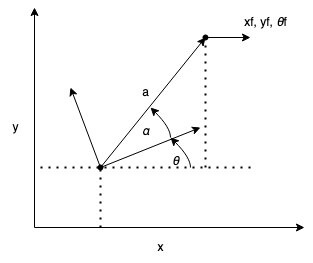
\includegraphics[scale=0.7]{graficos/grafico.png}
  \caption{Sistema}
\end{figure}

Así como el control no lineal, en éste paradigma también buscamos el control de nuestro robot. Por lo que el sistema támbien se puede representar con el mismo diagrama.

\begin{figure}[h]
  \centering
  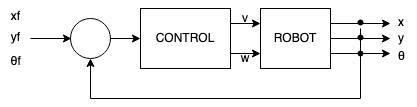
\includegraphics[scale=0.7]{graficos/bloque.png}
  \caption{Sistema de Control Difuso}
\end{figure}

\subsection{Definición de variables lingüisticas}

Nuestro dominio se muestra a continuación:
\begin{itemize}
\item Control de motores izquierdo (VL), derecho (VR) $VL \in (-100,100)$, $VR \in (-100,100)$.
\item Distancia de recorrido es variable (depende del $x_f$ y $y_f$), $a \in [0, \infty)$
\item Ángulo de error $\alpha \in (-\pi, \pi)$
\end{itemize}

\subsection{Construcción de base de reglas}

Se controlan 3 variables de salida.

Se parte de las reglas del experto. En está practica también se hace uso de la integración de odometría de practicas pasadas, para obtener la distancia recorrida por nuestro robot no holomico en todo instante.\\

Construcción de la base de conocimientos\\

Para nuestro motor derecho se tiene:
%Matriz
\begin{table}[h]
\centering
\begin{tabular}{l|l|l|l|l|}
\cline{2-5}
                         & Z & C   & L   & ML  \\ \hline
\multicolumn{1}{|l|}{ID} & 0 & -10 & -10 & -10 \\ \hline
\multicolumn{1}{|l|}{I}  & 0 & -10 & -10 & -10 \\ \hline
\multicolumn{1}{|l|}{Z}  & 0 & 10  & 20  & 30  \\ \hline
\multicolumn{1}{|l|}{D}  & 0 & 10  & 10  & 10  \\ \hline
\multicolumn{1}{|l|}{DD} & 0 & 10  & 10  & 10  \\ \hline
\end{tabular}
\end{table}

Para nuestro motor izquierdo se tiene:
%Matriz
\begin{table}[h]
\centering
\begin{tabular}{l|l|l|l|l|}
\cline{2-5}
                         & Z & C   & L   & ML  \\ \hline
\multicolumn{1}{|l|}{ID} & 0 & 10 & 10 & 10 \\ \hline
\multicolumn{1}{|l|}{I}  & 0 & 10 & 10 & 10 \\ \hline
\multicolumn{1}{|l|}{Z}  & 0 & 10  & 20  & 30  \\ \hline
\multicolumn{1}{|l|}{D}  & 0 & -10  & -10  & -10  \\ \hline
\multicolumn{1}{|l|}{DD} & 0 & -10  & -10  & -10  \\ \hline
\end{tabular}
\end{table}

Las potencias de los motores se pueden ajustar para tener un mejor desempleño, en nuestro caso se tiene un comportamiento lento que se puede correguir aumentando los numeros en el rando de dominio de los motores. 


\subsection{Fuzzificar, inferencia, defusificar}

Las membrecias se definen como el gráfico de distancia.

\begin{figure}[h]
  \centering
  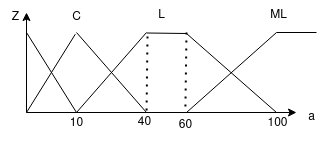
\includegraphics[scale=0.7]{graficos/fuzzy_distancia.png}
  \caption{Distancia}
\end{figure}

\begin{itemize}
\item Z - Zero
\item C - Cerca
\item L - Lejos
\item ML - Muy Lejos
\end{itemize}

\newpage
y su inclinación respecto al $x_f,y_f$ destino.

\begin{figure}[h]
  \centering
  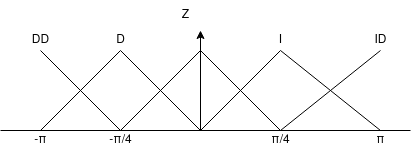
\includegraphics[scale=0.7]{graficos/fuzzy_orientacion.png}
  \caption{Orientación}
\end{figure}

\begin{itemize}
\item ID - Izquierda Detrás
\item I - Izquierda
\item Z - Zero (de frente)
\item D - Derecha
\item DD - Derecha Detrás
\end{itemize}

Apartir de los conocimientos vertidos en se puede obtener la distancia para cada instante respecto al desplazamiento del robot:

\SetKwComment{Comment}{/* }{ */}

\begin{algorithm}[H]
\caption{Desplazamiento}\label{alg:one}
\uIf{a < 10}{
  $z \gets 1 - (a/10)$;\\
  $c \gets a/10$;\\
  $l \gets 0; ml \gets 0$;\\
}\uElseIf{a<50}{
  $z \gets 0$;\\
  $c \gets 1-((a-10)/40)$;\\
  $l \gets ((a-10)/40); ml \gets 0$;\\
}\uElseIf{a<100}{
  $z \gets 0$;\\
  $c \gets 0$;\\
  $l \gets (1-((a-50)/50)); ml \gets ((a-50)/50)$;\\
}\Else{
  $z \gets 0$;\\
  $c \gets 0$;\\
  $l \gets 0; ml = 1$;\\
}
\end{algorithm}


Para la inclinación $DD \gets -\pi$, $D \gets \frac{-\pi}{4}$, $Z \gets 0$, $I \gets \frac{\pi}{4}$, $DI \gets \pi$:

\begin{algorithm}[H]
  \uIf{$\alpha < D$}{
    $MD \gets \frac{\alpha-D}{D-DD}$\;
    $MDD \gets 1-MD$\;
    $MZ \gets 0$\; $MI \gets 0$\; $MDI \gets 0$\;
  }
  \uElseIf{$\alpha < Z$}{
    $MZ \gets \frac{\alpha-D}{Z-D}$\;
    $MD \gets 1-MZ$\;
    $MDD \gets 0$\; $MI \gets 0$\; $MDI \gets 0$\;
  }
  \uElseIf{$\alpha < I$}{
    $MI \gets \frac{\alpha-Z}{I-Z}$\;
    $MZ \gets 1-MI$\;
    $MDD \gets 0$\; $MD \gets 0$\; $MDI \gets 0$\;
  }
  \Else{
    $MDI \gets \frac{\alpha-I}{DI-I}$\;
    $MI \gets 1-MDI$\;
    $MDD \gets 0$\; $MD \gets 0$\; $MZ \gets 0$\;
  }
\caption{Inclinación}
\end{algorithm}

\newpage
Apartir de los valores obtenidos de distancia e inclinación se calcula la potencia de los motores

\SetKwFor{For}{for (}{) $\lbrace$}{$\rbrace$}

\begin{algorithm}
  \For{$i = 0;\ i < 4;\ i = i++$}{
    \For{$j = 0;\ j < 5;\ j = j++$}{
      \uIf{$MA[i]<MAlpha[j]$}{
        $coef = MA[i]$\;
      }\uElse{}{
        $coef = MAlpha[j]$\;
      }
      $acc\_coef = acc\_coef + coef$\;
      $acc\_accion = acc\_accion + coef * VL[j][i]$\;
    }
  }
  $accion\_VL = \frac{acc\_accion}{acc\_coef}$
  \caption{Potencia para motor Izquierdo}
\end{algorithm}

\begin{algorithm}
  \For{$i = 0;\ i < 4;\ i = i++$}{
    \For{$j = 0;\ j < 5;\ j = j++$}{
      $coef2 = min(MA[i],MAlpha[j])$\;
      $acc\_coef2 = acc\_coef2 + coef2$\;
      $acc\_accion2 = acc\_accion2 + coef2 * VR[j][i]$\;
    }
  }
  $accion\_VR = \frac{acc\_accion2}{acc\_coef2}$
  \caption{Potencia para motor Derecho}
\end{algorithm}


\newpage
\section{Resultados}

El comportamiento que se obtuvo representó un desplazamiento como el siguiente gráfico. Mostrando la corrección de $\alpha$ desde su inicio, para comenzar la navegación.\\

Se puede observar un pequeño video de la demostración del trabajo. \href{https://youtube.com/shorts/GgrXnc17P5M?feature=share}{ver video}

\begin{figure}[h]
  \centering
  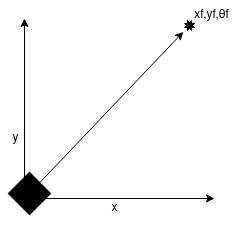
\includegraphics[scale=0.7]{graficos/fuzzy_control.png}
  \caption{Desplazamiento del robot móvil}
\end{figure}

Nuevamente, nuestro robot puede presentar errores sistematicos como derrapes, u obstáculos dentro de nuestro camino. Así como potencias bajas en los motores apreciando un desplazamiento nulo, este último se puede correguir reasignando nuevos valores a nuestra matriz de conocimientos.\\

Ver códigos fuentes \href{https://github.com/luisballado/MobileRobotics/blob/765b278bdd76b460300f6093620ef75676cff66e/codes/fuzzy.nxc}{github}

%------------------------------------------------
\section{Conclusiones}

La implementación del un control difuso nos brinda grandes ventajas, pero solo es interpolador. Fuera de los rangos a controlar no obtendremos una solución.

En conclusión, el control difuso tipo Sugeno es una técnica de control basada en la lógica difusa que se diferencia del control difuso tipo Mamdani en que las reglas difusas definen funciones lineales en lugar de funciones de pertenencia. En este tipo de control, las entradas se transforman en valores lingüísticos mediante funciones de pertenencia, y se definen reglas difusas que se traducen en funciones lineales para cada variable de salida.

El control difuso Sugeno es útil en aplicaciones donde la precisión es fundamental y las variables de entrada tienen una relación lineal con la salida. Su capacidad para modelar sistemas no lineales de manera más precisa que el control difuso Mamdani lo hace adecuado para aplicaciones que requieren una alta precisión, como en el control de procesos industriales.

Sin embargo, el control difuso Sugeno puede resultar más difícil de diseñar que el control difuso Mamdani debido a la necesidad de definir funciones lineales para cada variable de salida. Además, la interpretación de los resultados puede resultar más difícil debido a la naturaleza lineal de las funciones de salida.

En resumen, el control difuso Sugeno es una técnica de control poderosa y efectiva en aplicaciones donde la precisión es fundamental y las variables de entrada tienen una relación lineal con la salida. Aunque puede presentar algunas dificultades en el diseño y la interpretación, su capacidad para modelar sistemas no lineales de manera más precisa lo hace una herramienta valiosa en el campo del control automático.


%----------------------------------------------------------------------------------------
%	REFERENCE LIST
%----------------------------------------------------------------------------------------

\begin{thebibliography}{2} % Bibliography - this is intentionally simple in this template

\bibitem{InstNXC} Intalación NXC en LINUX, \url{http://ubuntudaily.blogspot.com/2011/03/using-lego-mindstorms-nxt-with-ubuntu.html}
\bibitem{NBC} Repositorio Compilador NBC utilizado, \url{https://github.com/pierre-24/nbc-compiler}
\bibitem{avoidSudo} Documento para evitar sudo en NXC, \url{https://bricxcc.sourceforge.net/nbc/doc/nxtlinux.txt}
\bibitem{libusb} Comando para instalar libusb-dev, \url{https://howtoinstall.co/en/libusb-dev}
\bibitem{Odom} Presentación Odometría, \url{http://www.kramirez.net/Robotica/Material/Presentaciones/Odometria.pdf}
\bibitem{ModCin} Modelo Cinemático de un robot móvil tipo diferencial y navegación a partir de la estimación odométrica,\url{https://www.redalyc.org/pdf/849/84916680034.pdf} VALENCIA V., JHONNY A.; MONTOYA O., ALEJANDRO; RIOS, LUIS HERNANDO
\bibitem{MoCin} Modelo cinemático de un robot móvil implementado con LEGO NXT para un sistema de localización indoor diseñado en Labview, \url{https://www.google.com/url?sa=t&rct=j&q=&esrc=s&source=web&cd=&cad=rja&uact=8&ved=2ahUKEwiu0_So28_9AhViDkQIHRlXDtcQFnoECBQQAQ&url=https%3A%2F%2Frevistas.udistrital.edu.co%2Findex.php%2FTecnura%2Farticle%2Fdownload%2F6810%2F8394%2F30717&usg=AOvVaw2PsCrkFGkk_nGN-G084B11}
\bibitem{classNotes} Notas de clase, Robótica Móvil Inteligente, Dr. José Gabriel Ramírez Torres, Enero-Abril 2023  
\end{thebibliography}

%----------------------------------------------------------------------------------------

\end{document}
